\documentclass{article}
\usepackage[utf8]{inputenc}
\usepackage[margin=1.25in]{geometry}
\usepackage{graphicx}
\let\vec\mathbf

\title{The Camera Model}
\author{ Luke Thistlethwaite }
\date{October 2020}

\begin{document}

\maketitle

\section{Introduction}
Computer vision seeks to automate the process of human vision through computational, mathematical, and physics-based techniques. Its has numerous, interdisciplinary applications, ranging from manufacturing to medicine.

Computer vision is an \textit{inverse problem}: given insufficient visual information, construct a model to determine some unknowns, which could be a higher quality image or locating a region of interest.


\section{3-D World}
We live in a 3D world where every location is specified by three coordinates (X,Y,Z). Analogously, computer vision models place a camera and the surrounding objects in a 3D right-handed coordinate system. The images the camera captures is a 2D projection of the 3D space, and every pixel is specified by two coordinates (X,Y). The camera and objects are often translated and rotated. This is the subject of the next lecture.  

\section{Image Formation}
The images the camera captures depends on lighting, surface properties, scene geometry, and lens optics. One should always keep these factors in mind when before applying computer vision. We will return to many of these concepts when we discuss computer graphics. 

\subsection{Lighting}
Light sources in a scene are responsible for visibility and illumination. Emitted light bounces off surfaces and some eventually reach the lens of the camera.

\begin{center}
    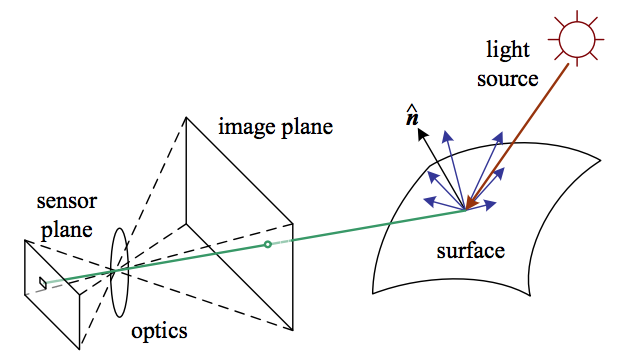
\includegraphics[height=1.5in, width=3in]{L1F2}\\ 
    \caption{How images form}
\end{center}
\\
Light scattering is modeled by a Bidirectional Reflectance Distribution Function (BDRF). A BDRF takes an input direction and returns the proportion of light reflected in an output direction at point $\vec{p}$. Because of the physics of light, swapping the input and output directions yields the same result.

$$ BDRF = f(\vec{p},\vec{w_i},\vec{w_o}) $$ 
\noindent 
To determine the amount of light reflected in a given a direction given an input direction, we can multiply the BDRF with the amount of incoming light in that direction times the \textit{foreshorting term}, which accounts for a decrease in reflectance as the angle between $\theta_i$ the incoming light and surface normal is increased. This is because the surface area exposed to the light is larger at oblique angles, and less light intensity is concentrated at a point.

$$ L(\vec{p},\vec{w_o}) = L(\vec{p},\vec{w_i})f(\vec{p},\vec{w_i},\vec{w_o})cos^+(\theta_i)$$
$$ cos^+(\theta_i) = max(0, cos(\theta_i))$$
\noindent
Given many input directions, we can write:

$$ L(\vec{p},\vec{w_o}) = \sum_{i} L(\vec{p},\vec{w_i})f(\vec{p},\vec{w_i},\vec{w_o})cos^+(\theta_i)$$
 \noindent
And taking into account incoming light from the entire surroundings, we can write:
$$ L(\vec{p},\vec{w_o}) = \int L(\vec{p},\vec{w_i})f(\vec{p},\vec{w_i},\vec{w_o})cos^+(\theta_i)d\vec{w_i}$$
\noindent
BDRF for a surface are usually obtained by physical modeling. Many BDRFs can be split into \textit{diffuse} and \textit{specular} components, allowing us to compute it easily.

\subsubsection{Diffuse}
The diffuse component accounts for shading. It scatters light uniformly  in all directions, so the diffuse component of the BDRF is constant at $\vec{p}$.

$$ L_d(\vec{p},\vec{w_o}) = \int L(\vec{p},\vec{w_i})f_d(\vec{p})cos^+(\theta_i)d\vec{w_i}$$ 

\subsubsection{Specular}
The specular component accounts for glossy reflections. Instead of scattering light, it reflects a single beam. The output direction thus has the same angle as the incoming light by Law of Reflection. Note the models define $f_s$ as dependent on the angle, so we do not have to multiply it with the foreshorting term. For instance, the Phong BDRF defines $f_s$ to be a power of the cosine angle. 

$$\vec{s_i} = \vec{v_{\parallel}} - \vec{v_{\perp}}$$
$$L_s(\vec{p}, \vec{w_o}) = \int L(\vec{p},\vec{w_i})f_s(\vec{p})d\vec{w_i}$$

\begin{center}
    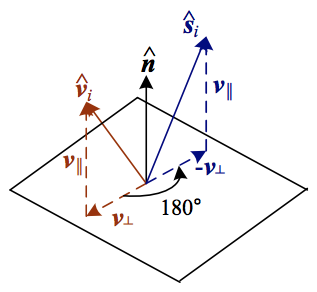
\includegraphics[height=1.3in, width=1.5in]{L1F4} \\
    \caption{Law of Reflection}
\end{center}
\\

\subsection{Lens Optics}
After light reaches the camera, it must past through the lens.

\subsubsection{Pinhole Camera Model}
Usually it is sufficient to model the camera aperture, the location that allows the light through, as a pinhole. This means that all light rays that hit the camera converge at one focal point, so the image is simply a scaled 2D projection of the 3D space. This projection is known as a perspective transformation, and it along with other transformations will be covered in the next lecture. Notice in diagram 2, the pinhole is behind the image place. This is because by the location of the image plane behind the pinhole is just the front image plane flipped upside-down. 

\begin{center}
    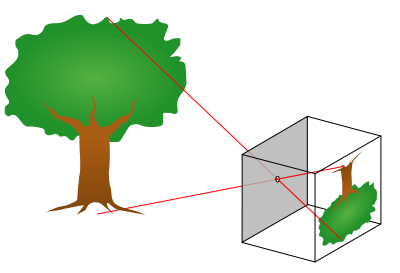
\includegraphics[height=1.5in, width=2in]{L1F6}
    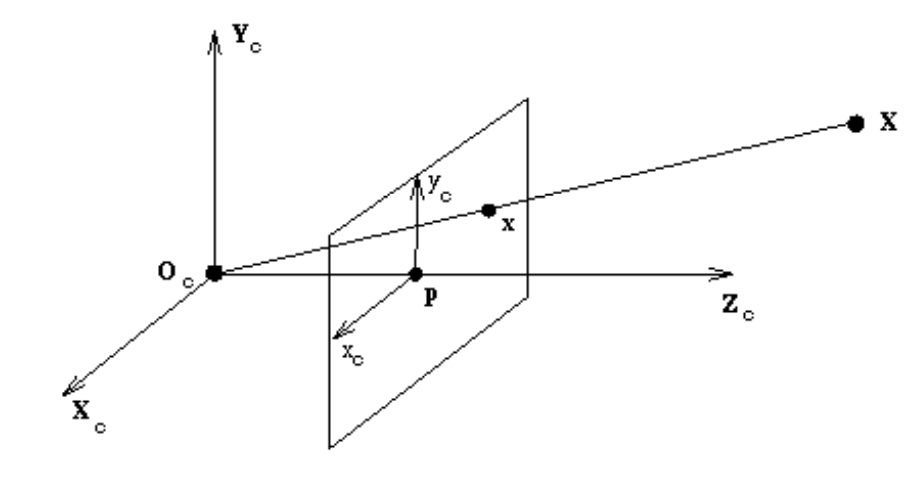
\includegraphics[height=1.5in, width=2in]{L1F5} \\
    \caption{Pinhole Camera Model; Perspective Projection}
\end{center}
\\ \\ 
However, if we want to account focus, exposure, etc, we must account for the lens.

\subsubsection{Thin Lens Focus}
Assume we have a thin convex lens. Let us define the distance the horizontal distance (z-axis in the diagram) of the object from the lens as $S_1$ and the distance from the lens to the plane to where the image formed is focused $S_2$. We also define the distance from the lens to the focus of the lens as $f$. In a pinhole camera, although there is no lens, we define $f$ = $S_1$.

Because our lens is thin, by the thin lens approximation, rays passing through the center of the lens are not refracted. Thus, we can derive the relationship:

$$ \frac{1}{f} = \frac{1}{S_1} + \frac{1}{S_2}$$ \\
\noindent
If the focal plane is moved away from the ideal position, the a fuzzy \textit{circle of confusion} results. The acceptable range of object locations given a image plane setting is known as the \textit{depth of field}. Pinhole cameras have an infinite depth of field.

As the object is moved towards $\infty$, note that $f$ = $S_1$, which is exactly the property of the pinhole camera. This is because the light rays straighten out and become parallel, and the lens results in a pinhole camera.

\begin{center}
    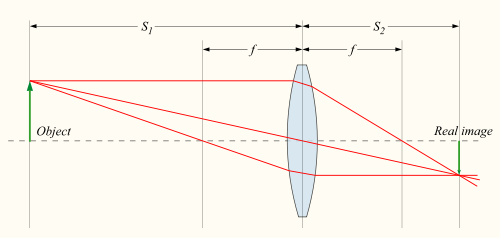
\includegraphics[height=1.2in, width=3.75in]{L1F7} \\
    \caption{Simple Lens Law Schematic}
\end{center} \\ \\ 

\section{The Digital Camera}
Finally the light has reached the part of the camera that will capture the image in digital memory! Photons are picked up by the \textit{active sensing area}, integrated into an representation for a exposure duration (camera parameter) by the \textit{shutter}, and finally passed through a set of processes to yield the final result.    

\begin{center}
    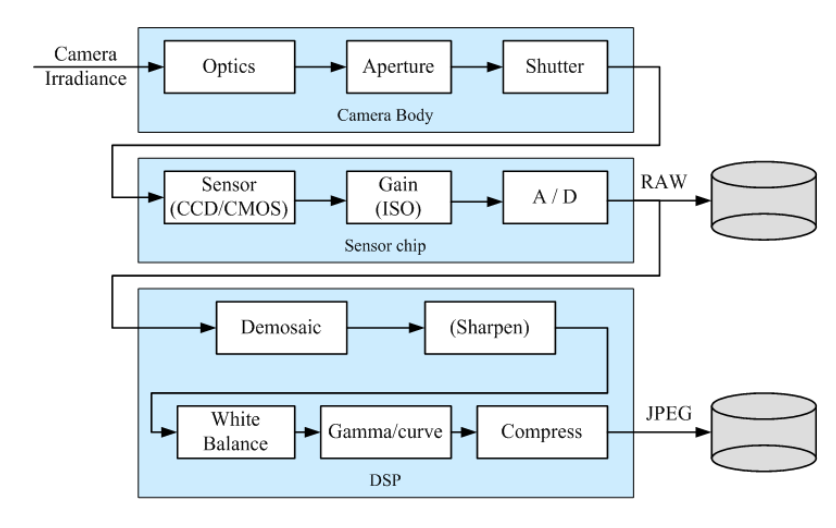
\includegraphics[height=1.75in, width=2.75in]{L1F8} \\
    \caption{The Digital Camera}
\end{center} \\ \\

\subsection{Color}
Images are composed of pixels of RGB values that specify a unique color. The digital camera must integrate different wavelengths of incoming light into discrete RGB values. In place of each pixel is a R,G, or B sensor. For instance, the Bayer arrangement:

\begin{center}
    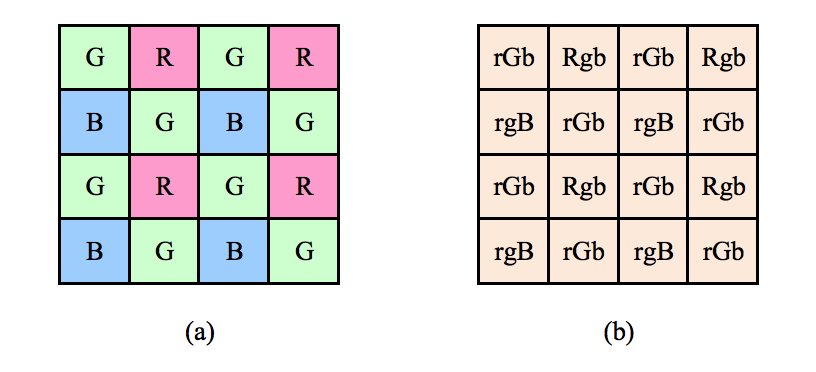
\includegraphics[height=1.25in, width=2.75in]{L1F10} \\
    \caption{(a)Bayer arrangement, (b) interpolated colors}
\end{center} \\ \\

\subsection{Compression}
The last step is to compress an image to save memory. There are many compression algorithms out there that are far beyond the scope of this lecture.

We take the time to introduce the \textit{peak signal-to-noise ration}. PSNR measures the quality of an image, which is a standard metric used during compression and many other cases:

$$ PSNR = 10log(\frac{I_{max}^2}{MSE})$$
\noindent
where MSE is the mean squared error of image and $I_{max}$ is the maximum possible signal value (255 for 8-bit images). 

$$ MSE = \frac{1}{n}\sum_{i}[I(i)-\hat{I(i)}]^2$$
\noindent
where $n$ is the number of pixels, $I(i)$ is the pixel value of the uncompressed image, and $\hat{I(i)}$ is the value of its compressed counterpart. PSNR is used in assessing image quality in signal processing, computer vision, computer graphics, and computational photography. 






\end{document}
